\chapter{\label{CH:Pipeline}TuMag's pipeline and data.}
INtro? tumag flew on bla vla. The data was recovered bla bla,
The reduction process started on bla bla and is ongoing right now bla bla. 

\section{TuMag's observing modes}

TuMag operates through a series of so-called observing modes. The observing modes are a list of pre-configured settings for the observations that fullfill different scientific puprposes and are meant to allow an almost automatic operation of the instrument during flight. 

\begin{table}
    \centering
   \begin{tabular}{cccccccc}
    \hline
    \hline
    Observing mode & Spectral lines  & $N_\lambda$ & $N_P$ & $N_a$& $N_c$ & $t_{eff} (s)$ & (S/N) \\
    \hline
    0s & Mg I $b_2$ 5172.7 \r{A} & 12 & 1 & 2 & 1 & 6.3 & 500\\ 
    0p & Mg I $b_2$ 5172.7 \r{A} & 12 & 4 & 16 & 1 & 37.62 & 1000\\
    1  & Mg I $b_2$ 5172.7 \r{A} &  10 & 4 & 16 & 1 & 31.81 & 1000\\
    2  & Fe I 5250.2 \r{A}, Fe I 5250.6 \r{A} &  8 & 4 & 16 & 1 & 23.4 & 1000\\
    3  & Fe I 5250.2 \r{A}, Fe I 5250.6 \r{A} & 5 & 2 & 20 & 1 & 10.04 & 1000\\
    4  & Mg I $b_2$ 5172.7 \r{A} & 3 & 4 & 10 & 10 & 54.01 & 2500\\
    5  & Fe I 5250.2 \r{A}, Fe I 5250.6 \r{A} & 3 & 4 & 10 & 10 & 53.60 & 2500\\ 
    \hline
    \hline
    \end{tabular}
    \caption{Scientific observing modes. From left to righ, the columns are: observing mode identiicator, measured spectral lines, number of wavelengths, of modulations, of accumulations, of cycles, the total timeand the polarimetric SNR.}
    \label{table: scientific observing modes}
\end{table}

A summary of the properties for each observing mode is provided in Table \ref{table: scientific observing modes}. There are four distinct modes designed to observe the magnesium line. Mode 0s performs a fast, extended scan of the spectral line using 12 wavelength samples: [-40, -30, -20, -10, 0, 10, 20, 30, 40, 50, 60, 65]\footnote{Sampling positions are given relative to the line core.}, with one modulation and two accumulations to maximize scanning speed. Mode 0p is similar to mode 0s but employs a full-vector modulation scheme, requiring 16 accumulations to ensure the required SNR. Mode 1 provides a shortened scan of the magnesium line, with measurements taken at [-30, -20, -10, -5, 0, 5, 10, 20, 30, 65], also utilizing a vectorial modulation scheme. Finally, mode 4 is a "deep" magnetic mode, featuring a highly reduced scan with only three samples at [-10, 0, 10], but with increased accumulations and cycles to enhance polarimetric sensitivity. 

Three observing modes are configured for the iron lines. Mode 2 employs a vectorial modulation scheme applicable to both iron lines, with sampling at [-12, -8, -4, 0, 4, 8, 12, 22] pm. Mode 3 uses a longitudinal modulation scheme, measuring only Stokes I and V, with samples taken at [-8, -4, 4, 8, 22] pm. Lastly, mode 5 closely resembles mode 4, but is configured for the iron lines, with sampling at [-8, 0, 8] pm. The only difference between these two modes is the sampling scheme.

Although most of the parameters are set up by the observing mode and cannot be changed, there are some configurable parameters that allow to slightly modify the observing modes to fit the specific goal of a particular. These parameters are the following:

Solo estos? o había más? 
\begin{itemize}
    \Myitem $\lambda _ {\text{rep}}$ : A parameter that allows to repeat all the observations carried out at every spectral position before changing wavelength. This parameter is employed for flat-field observations (see the following section). By default is set to 1.
    \Myitem Etalon offset : A parameter that allows for the introduction of a global shift to the spectral sampling by offsetting the absolute voltages (and thus, wavelengths) of the scan. This parameter was used to center the spectral line in shorter observing modes affected by solar rotation or other effects that might shift the spectral position. The default value is set to 0 V.
    \Myitem $N_a$ : Even though the number of accumulations is fixed in nominal observing modes, this parameter was set as configurable in order to allow modifications for faster observations when needed. The  default value depends on the observing mode.  
\end{itemize}

Figure \ref{fig_pipeline: Observing modes ranges} presents a schematic representation of the voltage ranges for the observing modes when converting spectral sampling to volts. The black lines indicate the voltage boundaries that cannot be surpassed during an observation due to technical constraints. These limits are set at $\pm 3750$ V as the maximum and minimum values, with an additional limitation at 0 V, since a polarity change poses technical challenges that could not be addressed within an observation mode. These restrictions are significant in two cases: firstly, for Magnesium observation modes, specifically modes 1 and 0, where the continuum measurement is positioned as far from the core as possible, at -80 V, due to the 0 V crossing limitation. Secondly, these constraints are relevant when applying an etalon offset to shift the spectral positions of a particular observing mode, as the offset cannot cause the final positions to exceed these boundaries.

\begin{figure}[t]
    \begin{minipage}[c]{0.67\textwidth}
      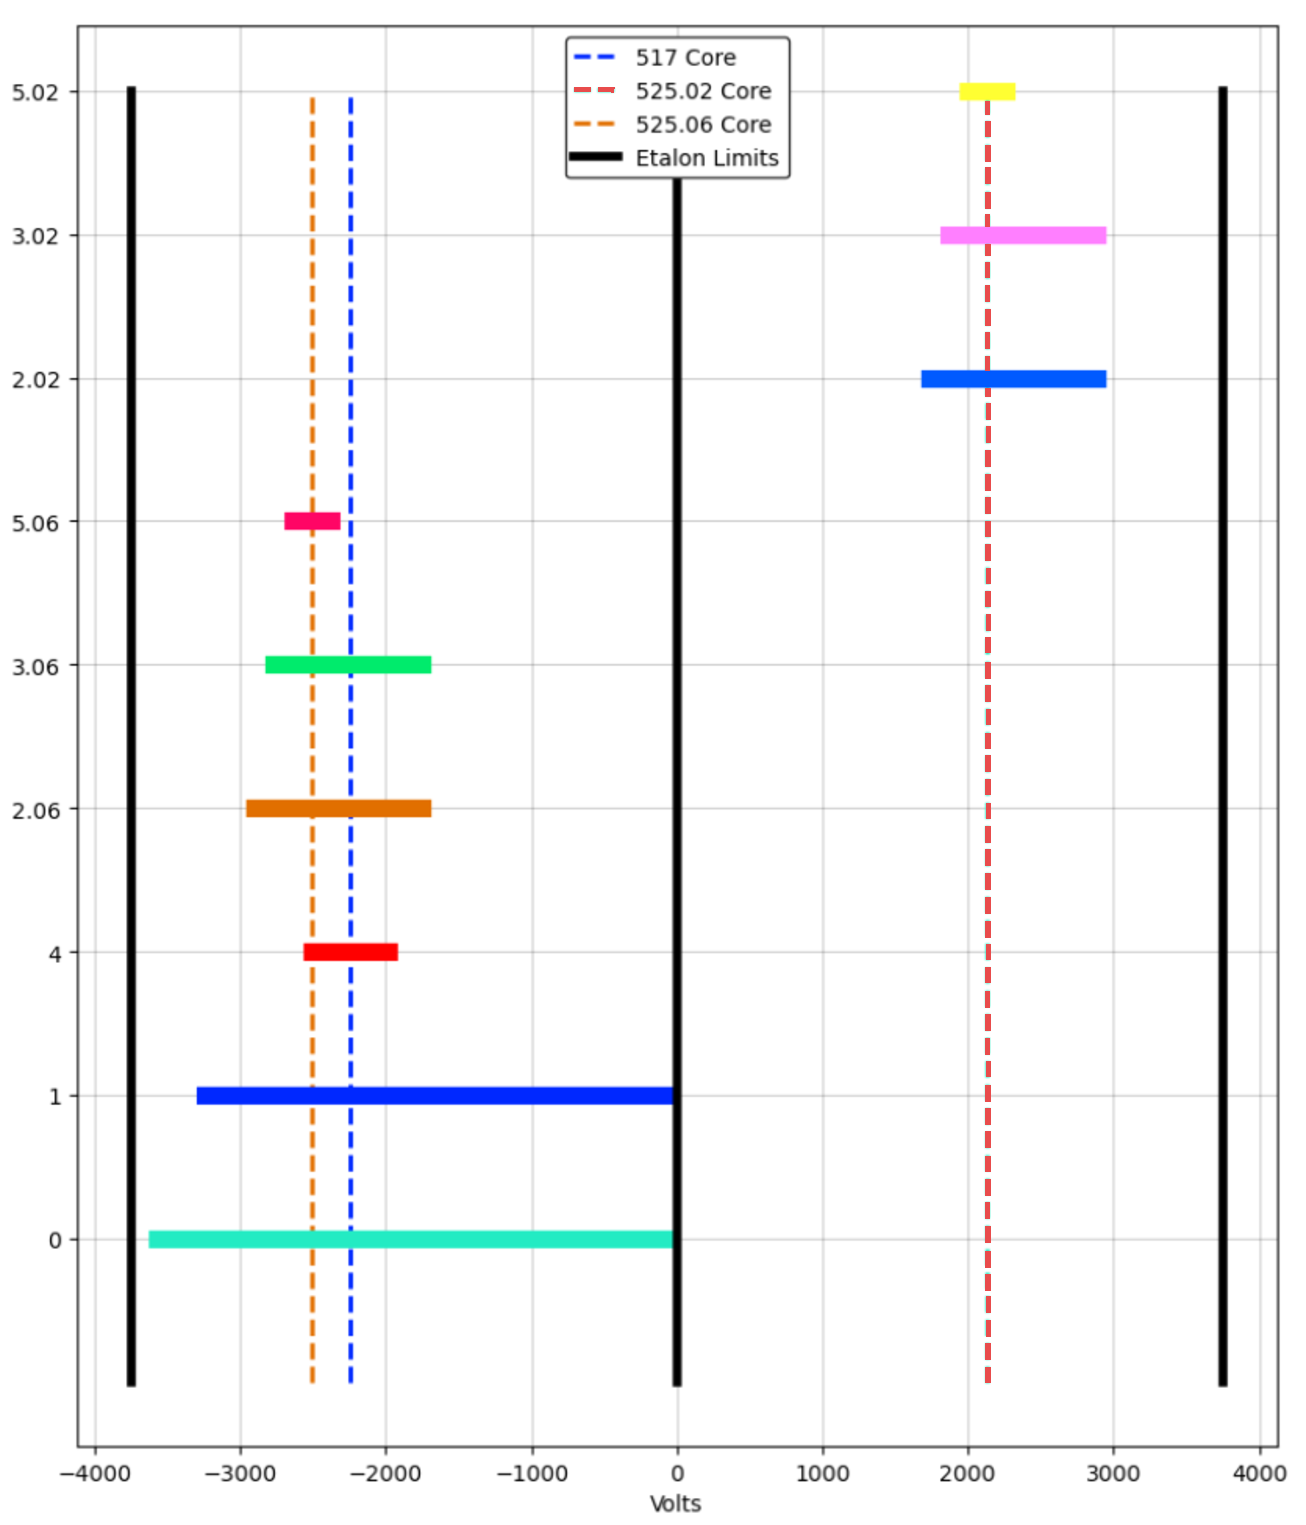
\includegraphics[width=\textwidth]{figures/Pipeline/obs_modes.pdf}
    \end{minipage}\hfill
    \begin{minipage}[c]{0.29\textwidth}
      \caption{
       Schematic representation of the voltage range covered by all observing modes. The dashed lines indicate the position of the line core as measured during the E2E tests performed at INTA in December 2021. The black lines represent the voltage limits that cannot be crossed in an observing mode.
       \label{fig_pipeline: Observing modes ranges}
      } 
    \end{minipage}
  \end{figure}


\subsection{Calibration modes}
An additional type of observing modes are also designed aimed at carrying out calibration observations. These calibration observing modes are more flexible than scientific ones, and allow for the configuration of several parameters to match the observations to the aim of the scientific observation. 

\begin{figure}[t]
    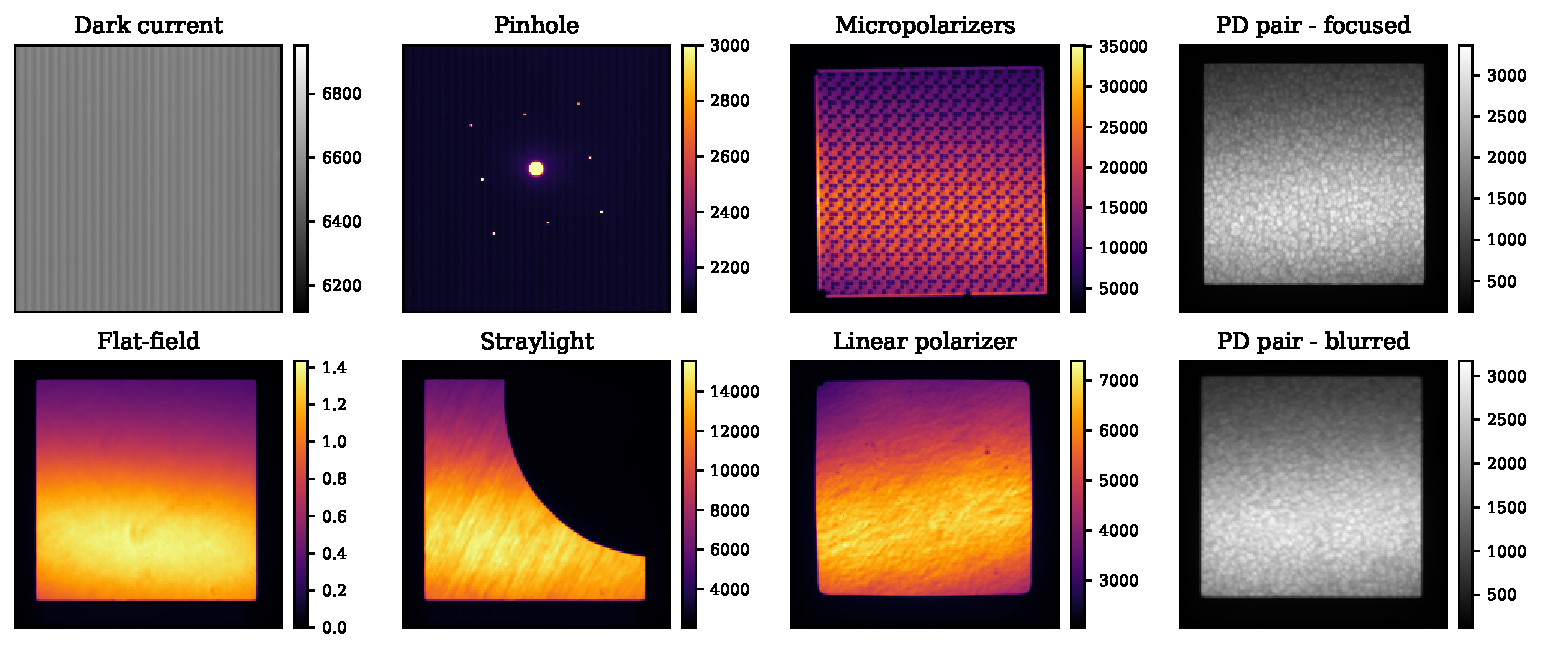
\includegraphics[width=\textwidth]{figures/Pipeline/cal_modes_examples.pdf}
    \caption{
      Examples of calibration observations. All images, with the exception of the flat-field, are presented in their raw format, without any manipulation or correction applied. The flat-field observation depicted corresponds to the first modulation of the continuum measurement obtained during a flat-field observation corresponding to observing mode 1. All data are belong to camera 1, and the colorbar is calibrated in digital counts save for the flat-field which is normalized to its mean value. }
      \label{fig_pipeline: cal_examples}
\end{figure}

\subsubsection{Flat-field observations}

One of the essential calibration procedures in any telescope-based astronomical observation is the acquisition of flat-field images. These observations are designed to measure intensity variations across the FoV, which arise from several factors, including intensity gradients induced by the etalon, dust particles, or pixel efficiency variations, among other sources. The aim is to capture a region with no discernible structure, ideally producing a uniformly flat intensity distribution. However, achieving such flat-field observations is not always straightforward, particularly for certain instruments. While ground-based telescopes can utilize twilight periods to observe areas of the sky devoid of stars, space-borne or balloon-borne solar telescopes, such as Sunrise III, are unable to the dame and must look for alternative methods. 

In Sunrise III, flat-field images are generated by deliberately blurring the solar image through rapid movements of the mirror. This process effectively removes any solar structure from the FoV when averaging out multiple blurred observations, resulting in a flat-field image devoid of solar features.

In the case of TuMag, flat-field observations are performed using a modified version of the nominal observing mode, where the $\lambda_{\text{rep}}$ is set to 4. Additionally, multiple consecutive instances ($N_{\text{reps}}$) of these observations are executed, typically 5 or 7. During data processing, a single flat-field is generated for each wavelength position and modulation state by averaging all corresponding observations.

Figure \ref{fig_pipeline: cal_examples} shows an example of a flat-field observation, for one camera, modulation and wavelength (bottom left panel). The image shows a clear deviation from flatness in the measurment, primarly due to the etalon intensity gradient, which accounts for the change in intensity between the brighter bottom half and the darker top half, and some minor inhomogeneities over the FoV. 

\subsubsection{Dark-current observations}

A second critical calibration procedure for any observation involving electronic cameras is the measurement of dark current. In the absence of incident photons, electrons within the camera's wells can still be randomly excited. This spontaneous excitation can be incorrectly interpreted as photon-induced counts when analyzing the data. Dark current observations are designed to characterize these random electronic excitations, which are primarily influenced by the camera's physical conditions, particularly temperature, so that they can be accurately subtracted from the final images.

For TuMag, dark current calibration involved capturing a series of 50 images with $N_a = 50$ with no light entering the instrument. As with flat-field observations, a single dark current frame for each camera is generated by averaging all individual observations. In the top left panel of fig. \ref{fig_pipeline: cal_examples} a dark current shot is depicted, characterized by the vertical strips pattern.  

\subsubsection{Linear polarizer and micropolarizers observations.}

TuMag's filter wheels are equipped with two targets designed to assess the instrument's polarimetric performance: a linear polarizer and a set of micropolarizers. Both targets are situated in the first filter wheel and are used in conjunction with the three distinct prefilters located in the second filter wheel. The linear polarizer serves to evaluate the polarimetric calibration, particularly by quantifying the level of cross-talk, as no circular polarization should be detected when using this target. The micropolarizers provide a more complete assessment, as they consist of multiple linear polarizers oriented at different angles. 

Observations with this targets are carried with the three prefilters, at a single wavelength, located in the continuum of each line. For each measurement, a vectorial modulation scheme is employed that allows for the derivation of the four stokes parameters. In the third column of figure \ref{fig_pipeline: cal_examples} observations of both targets are shown. 

\subsubsection{Pinhole Observations.}

Another calibration target included in the filter wheels is the pinhole target. This target blocks most of the light reaching the instrument, except for a few small holes arranged in a square-like pattern across the FoV, as shown in the top panel of the second column of figure \ref{fig_pipeline: cal_examples}. A larger hole is located at the center of the FoV, surrounded by eight smaller holes that trace a square with the central hole at its midpoint. These observations serve various purposes, including image alignment, detecting the presence of ghost images, or identifying etalon reflections, among other uses.

Pinhole observations are conducted similarly to those with polarizers, that is, in combination with the three prefilters at a single wavelength (the continuum of each line), but without applying any modulation.

\subsubsection{Straylight target.}

Not all the light that reaches the detector is necessarily the intended signal for a given observation. Some unwanted light, primarily originating from internal reflections along the optical path, may also reach the instrument. This unwanted contribution, known as straylight, contaminates the measurements by reducing contrast, lowering the S/N, and generally degrading the spectral, optical, and polarimetric performance of the instrument.

To address this contamination, TuMag performed a series of observations using a target that blocks part of the FoV (see the bottom panel of the second column of figure \ref{fig_pipeline: cal_examples}). By analyzing the dark region in these observations, it becomes possible to measure and model the straylight reaching the instrument, allowing for its subsequent removal from the data.

\subsubsection{Prefilter scans.}

TuMag observations are very sensible to spectral shifts either from the pre-filters or from the observed spectral line position. The shift of the pre-filters can happen due to changes in the physical conditions of the filter wheels such as changes in temperatures which spectraly shift the behavior of the pre-fitlers. The position of the pre-filter greatly affect the measurements as it reduces the intensity of the measurements that are obtained in the wings of the pre-filter. Due to solar rotation, or changes in the conditions of the etalon, although these are less likely, the spectral position at which the spectral lines are recorded can change. This effect is specially important in observing modes that require great spectral accuracy, such as the deep modes, where only three spectral positions close to the line core are employed. 

In order to verify the spectral behaviour of the prefilter, as well as the position of the spectral line, a series of observations were carried out, usually before and after the scientific observations, where a spectral scan with a rich spectral smapling was taken for all the pre-filters employed in the observation. These scans, measure the voltage range of the specific line with a sampling of \textcolor{red}{100V} and without modulating. 




\begin{figure}[t]
    \begin{minipage}[c]{0.67\textwidth}
      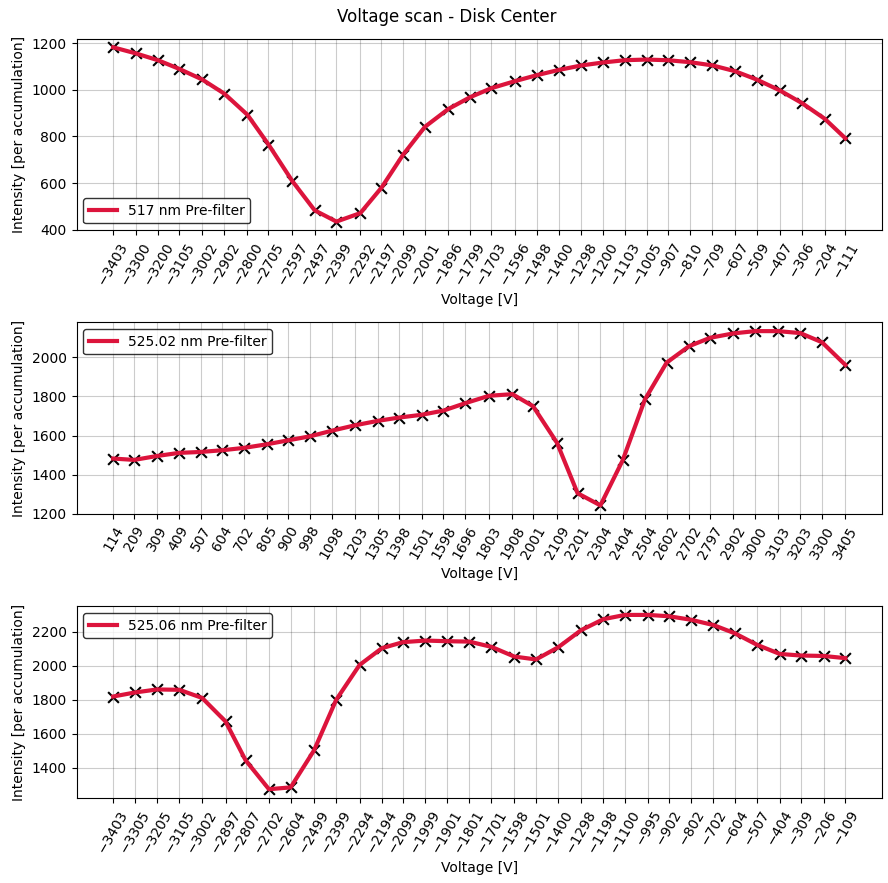
\includegraphics[width=\textwidth]{figures/Pipeline/Prefilter_scans.png}
    \end{minipage}\hfill
    \begin{minipage}[c]{0.29\textwidth}
      \caption{
       Schematic representation of the voltage range covered by all observing modes. The dashed lines indicate the position of the line core as measured during the E2E tests performed at INTA in December 2021. The black lines represent the voltage limits that cannot be crossed in an observing mode.
       \label{fig_pipeline:  prefilter_scans}
      } 
    \end{minipage}
  \end{figure}


\subsubsection{Phase diversity.}

Lastly, TuMag is equipped with the capability to perform phase diversity for image reconstruction. As discussed in previous chapters, applying image reconstruction techniques is essential to meet the optical quality requirements. To this end, TuMag includes a PD plate in the first filter wheel that introduces a known defocus in the images. Capturing images with and without this plate enables the computation of the instrument's PSF, which can then be deconvolved from the data.

PD measurements require quasi-simultaneous pairs of aberrated and unaberrated images. Therefore, TuMag's PD observations consist of a series of 32 or 40 rapid, non-accumulated shots with the PD plate, followed by a corresponding series without the PD plate. The feasibility of this sequential scheme for phase diversity techniques has been confirmed in \cite{PD_sequential}. A pair of focused-defocused images of quiet-sun observations is shown in the last column of figure \ref{fig_pipeline: cal_examples}.   


\section{Pipeline}
\subsection{Darks and flat fields}
\subsection{Blueshift}
\subsection{Demodulation and dual beam}
\subsection{Cross Talk}

